%%%%%%%%%%%%%%%%%%%%%%%%%%%%%%%%%%%%%%%%%
% Friggeri Resume/CV
% XeLaTeX Template
% Version 1.2 (3/5/15)
%
% This template has been downloaded from:
% http://www.LaTeXTemplates.com
%
% Original author:
% Adrien Friggeri (adrien@friggeri.net)
% https://github.com/afriggeri/CV
%
% License:
% CC BY-NC-SA 3.0 (http://creativecommons.org/licenses/by-nc-sa/3.0/)
%
% Important notes:
% This template needs to be compiled with XeLaTeX and the bibliography, if used,
% needs to be compiled with biber rather than bibtex.
%
%%%%%%%%%%%%%%%%%%%%%%%%%%%%%%%%%%%%%%%%%

\documentclass[]{luger-cv} % Add 'print' as an option into the square bracket to remove colors from this template for printing

\usepackage{fontspec}
\newfontfamily{\FA}[Path = fonts/]{fontawesome-webfont}

\usepackage{ragged2e}

\usepackage{marginnote}

\def\faEnvelope{{\FA\symbol{"F0E0}}}
\def\faGithub{{\FA\symbol{"F09B}}}
\def\faDesktop{{\FA\symbol{"F108}}}
\def\faPhone{{\FA\symbol{"F095}}}
\def\faHandPointerO{{\FA\symbol{"F25A}}}
\def\faMapMarker{{\FA\symbol{"F041}}}
\def\faVideoCamera{{\FA\symbol{"F03D}}}
\def\faCloudDownload{{\FA\symbol{"F0ED}}}

\input{citationskip}

\begin{document}

\header

%----------------------------------------------------------------------------------------
%	COORDINATES
%----------------------------------------------------------------------------------------

\aside{coordinates}{0.0325}{
    %
    \vspace*{-0.1cm}
    %
    \href{mailto:rodluger@gmail.com}{{\addfontfeature{Color=linkblue}rodluger@gmail.com}\ \faEnvelope}\\[0.5em]
    %
    \href{https://github.com/rodluger}{{\addfontfeature{Color=linkblue}github.com/rodluger}\ \faGithub}\\[0.5em]
    %
    \href{https://luger.dev}{{\addfontfeature{Color=linkblue}luger.dev}\ \faHandPointerO}\\[0.5em]
    %
    \href{tel:610-675-6056}{{\addfontfeature{Color=linkblue}+1 (610) 675 6056}\ \faPhone}\\[0.5em]
    %
    \href{https://www.google.com/maps/place/Center+for+Computational+Astrophysics/@40.7406078,-73.9906964,15z/data=!4m2!3m1!1s0x0:0xaa8b3847c99de596?sa=X&sqi=2&ved=2ahUKEwjk5bPEyp3dAhWqsKQKHUPgDkoQ_BIwDXoECAcQCw}{{\addfontfeature{Color=linkblue}\small Center for Computational }\\
        \href{https://www.google.com/maps/place/Center+for+Computational+Astrophysics/@40.7406078,-73.9906964,15z/data=!4m2!3m1!1s0x0:0xaa8b3847c99de596?sa=X&sqi=2&ved=2ahUKEwjk5bPEyp3dAhWqsKQKHUPgDkoQ_BIwDXoECAcQCw}{{\addfontfeature{Color=linkblue}\small Astrophysics, NY}}\ \faMapMarker}
    %
}

%----------------------------------------------------------------------------------------
%	EDUCATION
%----------------------------------------------------------------------------------------

\section{education}

\begin{entrylist}

    %------------------------------------------------

    \entry
    {2012--2017}
    {PhD {\normalfont Astronomy and Astrobiology}}
    {University of Washington, Seattle WA}
    {%
        \vspace{-1em}
        \begin{list}{{\color{numcolor}$-$}}{\cvlist}
            \item On the evolution, detection, and characterization of small \\ planets in the habitable zones of M dwarfs
            \item Advised by Eric Agol, Rory Barnes, and Victoria Meadows
        \end{list}
    }

    %------------------------------------------------

    \entry
    {2012--2013}
    {MSc {\normalfont Astronomy and Astrobiology}}
    {University of Washington, Seattle WA}

    %------------------------------------------------

    \entry
    {2006--2010}
    {BA {\normalfont Astrophysics}}
    {Swarthmore College, Swarthmore PA}
    {\vspace{-1em}
        \begin{list}{{\color{numcolor}$-$}}{\cvlist}
            \item Minor in English Literature
        \end{list}}

    %------------------------------------------------

\end{entrylist}

%----------------------------------------------------------------------------------------
%	ABOUT
%----------------------------------------------------------------------------------------

\aside{about}{0.0325}{
    \footnotesize
    \mbox{I~am~a~postdoctoral~fellow~at}
    \mbox{the~Center~for~Computational}
    \mbox{Astrophysics~in~New~York~City,}
    \mbox{working~on~finding~novel~ways}
    \mbox{to~discover~and~characterize}
    \mbox{exoplanets.~I~am~broadly~inter-}
    \mbox{ested~in~exocartography,~astro-}
    \mbox{statistics,~noise~modeling,}
    \mbox{\&~general~analytic~techniques}
    \mbox{for~astronomy.~Outside~of~the}
    \mbox{office~I~love~to~hike,~cycle,~swim,}
    \mbox{craft~lattes,~faulty~parallelism,}
    \mbox{and~Oxford~commas.}
}

%----------------------------------------------------------------------------------------
%	POSITIONS
%----------------------------------------------------------------------------------------

\section{positions}

\begin{entrylist}

    %------------------------------------------------

    \entry
    {2018--}
    {Flatiron Fellow}
    {Center for Computational Astrophysics, New York, NY}
    {%
        \vspace{-1em}
        \begin{list}{{\color{numcolor}$-$}}{\cvlist}
            \item Work on statistical and computational data analysis problems
                  \ifdefined \onepage \else
                      applied to stellar and exoplanetary astronomy
                  \fi
            \item Develop algorithms and open-source software for timeseries analysis
        \end{list}
    }

    %------------------------------------------------

    \entry
    {2017--2018}
    {Postdoctoral Researcher}
    {University of Washington}
    {%
        \vspace{-1em}
        \begin{list}{{\color{numcolor}$-$}}{\cvlist}
            \item Developed photometric de-trending methods to aid in the search for small
                  planets transiting small stars; developed and maintained the \texttt{everest} pipeline
        \end{list}
    }

    %------------------------------------------------

    \entry
    {2012--2017}
    {Research Associate}
    {University of Washington}
    {%
        \vspace{-1em}
        \begin{list}{{\color{numcolor}$-$}}{\cvlist}
            \item Developed techniques to detect and characterize habitable
                  zone planets
            \item Investigated the atmospheric evolution of planets orbiting M dwarfs
        \end{list}
    }

    %------------------------------------------------

    \ifdefined \onepage \else
        \entry
        {2008--2009}
        {Student Researcher}
        {Swarthmore College}
        {%
            \vspace{-1em}
            \begin{list}{{\color{numcolor}$-$}}{\cvlist}
                \item Research under Professor Eric Jensen on planet formation and T Tauri disks
            \end{list}
        }
    \fi

    %------------------------------------------------

\end{entrylist}

%----------------------------------------------------------------------------------------
%	STATS
%----------------------------------------------------------------------------------------

\aside{stats}{0.075}{
    \vspace*{0.5em}
    \input{pubs_summary}
}

%----------------------------------------------------------------------------------------
%	AWARDS
%----------------------------------------------------------------------------------------

\section{honors}

\begin{entrylist}

    \entry
    {2018--2022}
    {Flatiron Fellowship}
    {Center for Computational Astrophysics, New York, NY}
    {%
        \vspace*{-1.1em}
    }

    %------------------------------------------------
    \entry
    {2018}
    {Hubble Postdoctoral Fellowship}
    {(Declined)}
    {%
        \vspace*{-1.1em}
    }

    %------------------------------------------------

    \entry
    {2018}
    {51 Pegasi b Fellowship}
    {(Declined)}
    {%
        \vspace*{-1.1em}
    }

    %------------------------------------------------

    \entry
    {2012--2015}
    {ARCS Fellowship}
    {University of Washington}
    {%
        \vspace*{-1.1em}
    }

    %------------------------------------------------

    \entry
    {2010}
    {Bobby Berman Memorial Prize}
    {Swarthmore College}
    {%
        \vspace*{-1.1em}
    }

    %------------------------------------------------

    \ifdefined \onepage \else
        \entry
        {2010}
        {The Phi Beta Kappa Society}
        {Swarthmore College}
        {}
    \fi

    %------------------------------------------------

\end{entrylist}

%----------------------------------------------------------------------------------------
%	REFS
%----------------------------------------------------------------------------------------

\aside{references}{0.0325}{
    \textbf{eric agol}\\
    {\footnotesize agol@uw.edu}\\[0.3em]
    \textbf{david w. hogg}\\
    {\footnotesize dhogg@flatironinstitute.org}\\[0.3em]
    \textbf{rory barnes}\\
    {\footnotesize rory@astro.washington.edu}
}

%----------------------------------------------------------------------------------------
%	METRICS
%----------------------------------------------------------------------------------------

\ifdefined \onepage \else
    \section{metrics}

    % SUPER HACKY
    \raisebox{-0.9\height}[0pt][0pt]{
        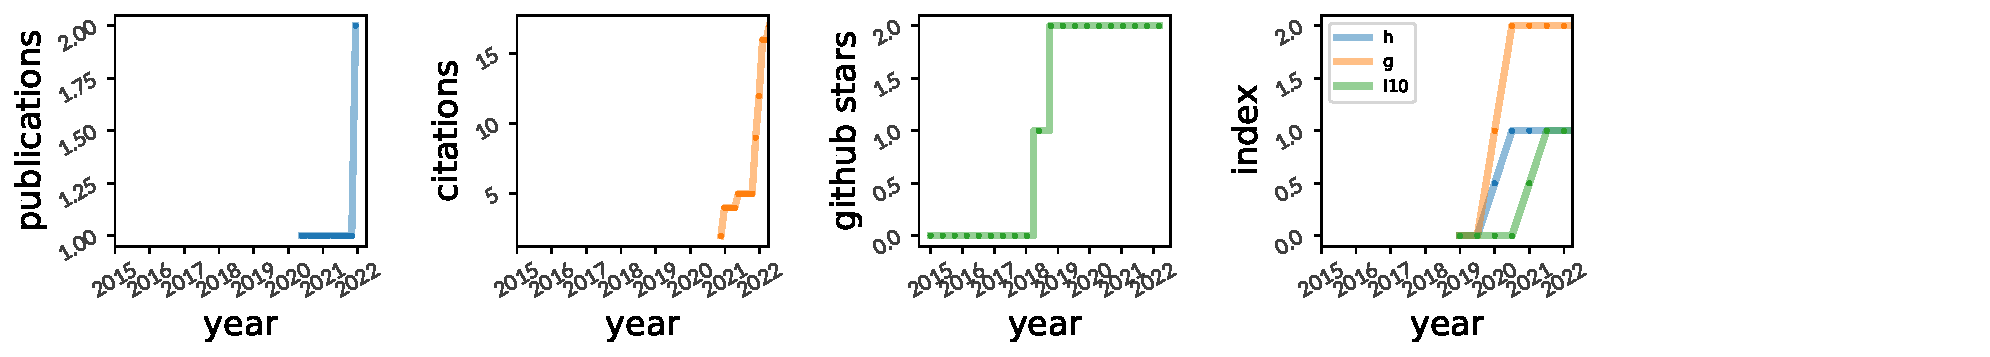
\includegraphics[height=1.25in]{metrics.pdf}
    }
    \pagebreak
\fi

%----------------------------------------------------------------------------------------
%	TEACHING
%----------------------------------------------------------------------------------------

\ifdefined \onepage \else
\aside{links}{0.05}{
    {\color{numcolor}\faVideoCamera} \, \link{https://tinyurl.com/wnxmxb43}{LSST Lecture I}\\[0.5em]
    {\color{numcolor}\faCloudDownload} \, \link{https://tinyurl.com/9247pj4}{LSST Worksheet I}\\[0.5em]
    {\color{numcolor}\faVideoCamera} \, \link{https://drive.google.com/file/d/1PW-5Tkwnai7uQAZB4COFBUVTgWMZkE1P/view?usp=sharing}{LSST Lecture II}\\[0.5em]
    {\color{numcolor}\faCloudDownload} \, \link{https://github.com/LSSTC-DSFP/LSSTC-DSFP-Sessions/tree/main/Session13/Day2}{LSST Worksheet II}\\[0.5em]
}
\fi
\section{teaching \& outreach}

\begin{entrylist}

    %------------------------------------------------

    \entry
    {2020-}
    {Mentor, Simons-NSBP Program}
    {Flatiron Institute}
    {%
        \vspace{-1em}
        \begin{list}{{\color{numcolor}$-$}}{\cvlist}
            \item Mentor black undergraduate students through the Simons-National
                  Society of Black Physicists summer program
        \end{list}
    }

    %------------------------------------------------

    \entry
    {2019-}
    {Mentor, AstroCom}
    {AMNH / CUNY}
    {%
        \vspace{-1em}
        \begin{list}{{\color{numcolor}$-$}}{\cvlist}
            \item Mentor undergraduate students from underrepresented groups in the sciences
                  at the City University of New York
        \end{list}
    }

    %------------------------------------------------

    \ifdefined \onepage \else

        \entry
        {2019-}
        {Lecturer, LSST Data Science Fellowship}
        {Carnegie Mellon / Flatiron Institute}
        {%
            \vspace{-1em}
            \begin{list}{{\color{numcolor}$-$}}{\cvlist}
                \item Lectured on various topics related to statistical
                      inference at week-long schools for early-career astronomers
            \end{list}
        }

        %------------------------------------------------

        \entry
        {2012--2017}
        {Mobile Planetarium}
        {University of Washington}
        {%
            \vspace{-1em}
            \begin{list}{{\color{numcolor}$-$}}{\cvlist}
                \item Presented planetarium shows at schools and public venues throughout
                      Washington state using UW's inflatable mobile planetarium
            \end{list}
        }

        %------------------------------------------------

        \entry
        {2012--2013}
        {Teaching Assistant}
        {University of Washington}
        {%
            \vspace{-1em}
            \begin{list}{{\color{numcolor}$-$}}{\cvlist}
                \item Taught two bi-weekly tutorial sessions for two college astronomy courses
            \end{list}
        }

        %------------------------------------------------

    \fi

    \ifdefined \onepage \else
\end{entrylist}
%
% PAGEBREAK
%
\begin{entrylist}
    \fi

    %------------------------------------------------

    \entry
    {2010--2012}
    {High School Teacher}
    {St. Luke's School, New Canaan CT}
    {%
        \vspace{-1em}
        \begin{list}{{\color{numcolor}$-$}}{\cvlist}
            \item Created and taught a rigorous, college-level elective course in astrophysics
                  aimed at seniors interested in pursuing college classes in the field
            \item Taught three sections of 11th grade physics with a focus on
                  astronomy
                  \ifdefined \onepage \else
                      , helping students develop critical thinking and creative
                      problem solving skills
                  \fi
        \end{list}
    }

    %

    \ifdefined \onepage \else
        \entry
        {2009--2010}
        {Science Associate \& Tutor}
        {Swarthmore College}
        {%
            \vspace{-1em}
            \begin{list}{{\color{numcolor}$-$}}{\cvlist}
                \item Directed weekly large-group study sessions for an introductory course in
                      astronomy; tutored students in courses in mechanics and E\&M
            \end{list}
        }
    \fi

    %------------------------------------------------

\end{entrylist}

%----------------------------------------------------------------------------------------
%	STUDENTS
%----------------------------------------------------------------------------------------


\ifdefined \withother

    \section{students}
    \begin{entrylist}

        %------------------------------------------------

        \entry
        {2020--}
        {Shashank Dholakia}
        {University of California, Berkeley}
        {%
            \vspace{-1em}
            \begin{list}{{\color{numcolor}$-$}}{\cvlist}
                \item Developing analytic transit light curve models for oblate stars
            \end{list}
        }

        %------------------------------------------------

        \entry
        {2020--}
        {Shishir Dholakia}
        {University of California, Berkeley}
        {%
            \vspace{-1em}
            \begin{list}{{\color{numcolor}$-$}}{\cvlist}
                \item Developing analytic transit light curve models for oblate stars
            \end{list}
        }

        %------------------------------------------------

        \entry
        {2020--2021}
        {Rebecca Young}
        {Simons-NSBP Scholars Program, CCA}
        {%
            \vspace{-1em}
            \begin{list}{{\color{numcolor}$-$}}{\cvlist}
                \item Inferring differential rotation rates from \emph{Kepler} light curves
            \end{list}
        }

        %------------------------------------------------

        \entry
        {2020--}
        {Fran Bartoli\'c}
        {Pre-doctoral Program, CCA}
        {%
            \vspace{-1em}
            \begin{list}{{\color{numcolor}$-$}}{\cvlist}
                \item Mapping the surface of Io from Jupiter occultation data
            \end{list}
        }

        \entry
        {2019--}
        {Asmaa Elsayed}
        {AstroCom Program, CUNY/CCA}
        {%
            \vspace{-1em}
            \begin{list}{{\color{numcolor}$-$}}{\cvlist}
                \item Understand the time evolution of spotted stellar surfaces
            \end{list}
        }

        \entry
        {2019}
        {Brynner Hidalgo}
        {AstroCom Program, CUNY/CCA}
        {%
            \vspace{-1em}
            \begin{list}{{\color{numcolor}$-$}}{\cvlist}
                \item Understand the time evolution of spotted stellar surfaces
            \end{list}
        }

        \entry
        {2016--2018}
        {Nicholas Saunders}
        {University of Washington}
        {%
            \vspace{-1em}
            \begin{list}{{\color{numcolor}$-$}}{\cvlist}
                \item Develop tools to mitigate systematics in \emph{K2} data
            \end{list}
        }

        %------------------------------------------------

    \end{entrylist}
\fi

\clearpage

%----------------------------------------------------------------------------------------
%	OTHER
%----------------------------------------------------------------------------------------

\ifdefined \withother

    \section{other}
    \begin{entrylist}

        %------------------------------------------------

        \entry
        {2018--}
        {Organizer, Stars and Exoplanets Meeting}
        {CCA}
        {%
            \vspace{-1em}
            \begin{list}{{\color{numcolor}$-$}}{\cvlist}
                \item Organize weekly meeting for NYC area graduate students, postdocs, \& faculty
            \end{list}
        }

        %------------------------------------------------

        \entry
        {2013--2017}
        {IT Manager}
        {Virtual Planet Laboratory, University of Washington}
        {%
            \vspace{-1em}
            \begin{list}{{\color{numcolor}$-$}}{\cvlist}
                \item Managed VPL's virtual conferencing system and network
            \end{list}
        }

        %------------------------------------------------

        \entry
        {2010--2012}
        {Head Coach}
        {St. Luke's School, New Canaan CT}
        {%
            \vspace{-1em}
            \begin{list}{{\color{numcolor}$-$}}{\cvlist}
                \item Head coach of the JV Boys Soccer and Fencing Teams
                      %\item Assistant coach of the MS Tennis Team
            \end{list}
        }

        %------------------------------------------------

    \end{entrylist}

    \aside{}{5.6}{
    {\footnotesize primary developer}\\[1em]
    \hrule
    {\footnotesize secondary developer}
    }
    \section{popular software}

    \begin{entrylist}

        %------------------------------------------------

        \entry
        {\textbf{starry}}
        {\textnormal{\texttt{pip install starry}}}
        {}
        {%
            \vspace{-1em}
            \begin{list}{{\color{numcolor}$-$}}{\cvlist}
                \item Tools for light curve modeling \& mapping stars and planets
            \end{list}
        }

        %------------------------------------------------

        \entry
        {\textbf{\scalebox{.85}[1.0]{starry-process}}}
        {\textnormal{\texttt{pip install starry-process}}}
        {}
        {%
            \vspace{-1em}
            \begin{list}{{\color{numcolor}$-$}}{\cvlist}
                \item Gaussian processes for modeling stellar variability
            \end{list}
        }

        %------------------------------------------------
        
        \entry
        {\textbf{\scalebox{.85}[1.0]{showyourwork}}}
        {\textnormal{\url{github.com/rodluger/showyourwork}}}
        {}
        {%
            \vspace{-1em}
            \begin{list}{{\color{numcolor}$-$}}{\cvlist}
                \item A workflow for open source, reproducible scientific articles
            \end{list}
        }

        %------------------------------------------------

        \entry
        {\textbf{planetplanet}}
        {\textnormal{\texttt{pip install planetplanet}}}
        {}
        {%
            \vspace{-1em}
            \begin{list}{{\color{numcolor}$-$}}{\cvlist}
                \item Tools for modeling planet-planet occultations
            \end{list}
        }

        %------------------------------------------------

        \entry
        {\textbf{everest}}
        {\textnormal{\texttt{pip install everest-pipeline}}}
        {}
        {%
            \vspace{-1em}
            \begin{list}{{\color{numcolor}$-$}}{\cvlist}
                \item Tools for de-trending \emph{K2} light curves\\[-0.5em]
            \end{list}
        }

        %------------------------------------------------

        \entry
        {\textbf{exoplanet}}
        {\textnormal{\texttt{pip install exoplanet}}}
        {}
        {%
            \vspace{-1em}
            \begin{list}{{\color{numcolor}$-$}}{\cvlist}
                \item Tools for probabilistic modeling of exoplanet time series data
            \end{list}
        }

        %------------------------------------------------

        \entry
        {\textbf{VPLANET}}
        {\textnormal{\texttt{pip install vplanet}}}
        {}
        {%
            \vspace{-1em}
            \begin{list}{{\color{numcolor}$-$}}{\cvlist}
                \item Suite for simulating planetary system evolution and habitability
            \end{list}
        }

        %------------------------------------------------

    \end{entrylist}
\fi

%----------------------------------------------------------------------------------------
%	PUBLICATIONS
%----------------------------------------------------------------------------------------

\ifdefined \withpubs
    %
    \ifdefined \citationskip
    \else
        \def\citationskip{0.95}
    \fi
    \aside{}{\citationskip}{
    {\footnotesize citations $\longrightarrow$}\\[0em]
    {\footnotesize (refereed in \textbf{bold})}
    }
    %
    \section{publications}
    %
    \begin{list}{}{\pubslist}
        \input{pubs}
    \end{list}
    %
    \vspace{1em}
    \clearpage
\fi

%----------------------------------------------------------------------------------------
%	TALKS
%----------------------------------------------------------------------------------------

%\clearpage

\ifdefined \withtalks

    \aside{}{0.95}{
        {\footnotesize {\color{numcolor}\faCloudDownload}\,: Downloadable}\\[0em]
        {\footnotesize {\color{numcolor}\faVideoCamera}\,: Watchable \phantom{XX.}}
    }
    \section{selected talks}
    %
    \begin{list}{}{\pubslist}
        \input{talks}
    \end{list}
\fi

\end{document}
